\documentclass[a4j,11pt]{article}


\newcommand{\doC}{^{\circ}{\rm C}}
\newcommand{\Do}{{}^{\circ}}
\newcommand{\mic}{\mu {\rm m}}
%\newcommand{\mob}{${\rm cm}^2{\rm V}^{-1}{\rm s}^{-1}$}
\newcommand{\mob}{{\rm cm}^2/{\rm V \mathchar"712D s}}
\newcommand{\sheet}{{\rm cm}^{-2}}
\newcommand{\bulk}{{\rm cm}^{-3}}
\newcommand{\alt}{~\raisebox{-0.6ex}{$\stackrel{\textstyle <}{\sim}$}~}
\newcommand{\agt}{~\raisebox{-0.6ex}{$\stackrel{\textstyle >}{\sim}$}~}

%% PDFファイルの作成方法
%
% ・dvipdfmを使う場合
%   dvipdfm -p A4 sample.dvi
%
% ・Adobe Acrobat (Distiller) を使う場合
%   dvipsk -D 600 -t a4 -P pdf sample.dvi
%   psファイルをDistillerでpdfへ変換
%

% ***************
%      注意!
% ***************
% 以下のtxfontsパッケージを使用するとcmフォントが(数式も含めて)Times,
% Helveticaなどに置き換えられます. % これを使いたくない方は以下の\usepackage{txfonts}を無効にしてください. 
% その場合にはcmフォントがPDFに埋め込まれるのでファイルサイズが多少大きくなります. 
%\usepackage{txfonts}

% 
% マージン設定(できるだけ変更しないでください)

% ######## measure #########
% # mm = 1mm = 2.85pt      #
% # cm = 10mm = 28.5pt     #
% # in = 25.4mm = 72.27pt  #
% # pt = 0.35mm = 1pt      #
% # em = width of [M]      #
% # ex = height of [x]     #
% # zw = width of [Kanji]  #
% # zh = height of [Kanji] #
% ##########################

\setlength{\textheight}{\paperheight}   % ひとまず紙面を本文領域に
\setlength{\topmargin}{-5.4truemm}      % 上の余白を20mm(=1inch-5.4mm)に
\addtolength{\topmargin}{-\headheight}  % 
\addtolength{\topmargin}{-\headsep}     % ヘッダの分だけ本文領域を移動させる
\addtolength{\textheight}{-50truemm}    % 下の余白も20mmに

\setlength{\textwidth}{\paperwidth}     % ひとまず紙面を本文領域に
\setlength{\oddsidemargin}{-5.4truemm}  % 左の余白を20mm(=1inch-5.4mm)に
\setlength{\evensidemargin}{-5.4truemm} % 
\addtolength{\textwidth}{-40truemm}     % 右の余白も20mmに

\pagestyle{empty}
\usepackage[dvipdfmx]{graphicx}
\usepackage{textcomp}
\usepackage[psamsfonts]{amssymb}
%\usepackage{mediabb}
\usepackage{here}

\usepackage{multirow} 
\makeatletter
\newcommand{\figcaption}[1]{\def\@captype{figure}\caption{#1}}
\newcommand{\tblcaption}[1]{\def\@captype{table}\caption{#1}}
\makeatother

\abovecaptionskip=0pt %図キャプション上部の余白の設定(標準:10pt)
\belowcaptionskip=0pt %図キャプション下部の余白の設定(標準:0pt)

\begin{document}
\renewcommand{\baselinestretch}{1.04}\small\normalsize %行間の間隔(標準:1)
%\setlength{\baselineskip}{0.5pt}

\begin{flushleft}
%Your presentation number
% A blank space is also acceptable.
\end{flushleft}

%\vspace{-12pt}
\begin{center}
\vspace{-5.5mm}
\textbf{\Large
インタラクティブ遺伝的アルゴリズムを用いた\\
プロシージャルモデリング支援システムの提案}
\end{center}

\begin{flushright}
\vspace{-2mm} 
\textbf{2210154}
\textbf{細川 岳大(Miyata Lab.)}
\end{flushright}

%%%%%%%%%%%%%%%%%%%%%%%%%%%%%%%%%
% Please feel free to write your own content. There is no need to write in sections as shown below. If you do not need a section at all, just insert % at the beginning of the line. The line will be ignored.
\vspace{-1mm}
\noindent
\textbf{[背景と目的, Background and purpose]}
\indent
近年ハードやソフトの技術進歩により, Computer Graphics(CG)の表現力が向上している.
CG 開発においてプロシージャルモデリングという手法がよく利用されており,数式や変数などをあらかじめ設定することで,変数のパラメータを変更するだけで様々なモデルを生成する事が出来る手法である.近年ハードやソフトの技術進歩による Computer Graphics(CG)の表現力向上のため,パラメータ数が多くなってきており,制作時間の増大が著しい.そこで本研究では,インタラクティブ遺伝的アルゴリズムを利用した操作パラメータ数を削減したシステムを提案し,制作時間短縮とユーザビリティ向上を目的とする.
\vspace{0.5mm}

\noindent{\bf [提案システム, Proposal system]}
\indent
図\ref{system}に提案システムを示す.操作手順について,まず6つの提案モデルから3つのモデルを選択する.次に3つのモデルの補間を三角形の平面UIで行う.そして,各パラメータの微調整を行い,最後に NEXT ボタンで提案モデルを更新する.この操作を繰り返して,自分の好きなモデルを生成する.この提案モデルを更新する際に,メタヒューリスティクスアルゴリズムであるインタラクティブ遺伝的アルゴリズム[1]を使用する.
\vspace{0.5mm}

\noindent{\bf [実験と結果, Experimental results]}
\indent
実験は2種類のタスクを設定しており,実験1は目標となるモデルの画像を見せてそれに近づけるタスク,実験2は目的を提示せず自由にモデリングするタスクである.また使用モデルのパラメータ数について,実験1は11,実験2は25のモデルを使用する.また対照実験として,ベイズ最適化を利用してモデル提案を行う研究[2]と比較する.


図\ref{fig:exp2AllTime}-\ref{fig:exp2StepTime}に実験2の結果を示す.操作時間全体では提案システムのほうが既存システムよりも時間はかかっている一方で,1ステップ当たりの時間やステップ数ではあまり差異が見られない.
図\ref{tSNE}にtSNEを用いてパラメータを二次元可視化したものを示す.青い縁取りが提案システム,赤い縁取りが対照実験による提案モデルであり,内部の色が 0 から 1 に行くにつれてステップ数が増加するようにしている.ステップ数が大きくなるほどに遺伝的アルゴリズムのほうがベイズ最適化よりも多様性を維持する事が出来,より広い探索が行えていることが確認できる.


またアンケート結果では,実験2のような多くのパラメータを持つモデルの自由なモデリングに関しては提案システムの有用性が高いという結果が得られた一方で,実験1のような目標が決まっている場合では既存システムのほうが有用性があるという結果になった.これは既存システムでは各パラメータをいつでも細かく調整できるため,目標の画像が見比べつつ行う事が出来たためである.対して,自由なモデリングは頭の中の想像に対して近づける必要があるため,細かいパラメータ調整より広く探索できる方がシステムとして優位性があるのではないかと考えられる.

\vspace{0.5mm}

\noindent{\bf [結論, Conclusions]}
\indent
本研究ではプロシージャルモデリングにおける操作性およびモデリング時間の改善のた
め,インタラクティブ遺伝的アルゴリズムにおけるモデル提案と平面 UI による補間を用いたモデリング支援システムを提案した.
平面 UI によって3つのモデルから補間されることにより直感的な操作で広い空間の探索を行うことができ,ユーザビリティ向上に繋がった.ユーザスタディの結果,定量評価では既存手法に比べ時間的優位性を見出すことはできなかったが, 定性評価から, 自由かつ多くのパラメータが存在するときには有用性は確認できた. 一方でインタラクティブ遺伝的アルゴリズムの有効性を確認することはできなかったため,最適なモデル提案手法が今後の課題である.

\vspace{1.5mm}

\noindent{\bf [Reference]}
\indent \small{[1] Janos Madar, Janos Abonyi, and Ferenc Szeifert. Interactive evolutionary computation in process engineering. Computers Chemical Engineering, 29(7):1591–
1597, 2005.  [2] Yuki Koyama and Masataka Goto. Bo as assistant: Using bayesian optimization
for asynchronously generating design suggestions. In Proceedings of the 35th
Annual ACM Symposium on User Interface Software and Technology, pages 1–
14, 2022.  [3] Laurens Van der Maaten and Geoffrey Hinton. Visualizing data using t-sne.
Journal of machine learning research, 9(11), 2008.


%\clearpage
\vspace{3mm}
\begin{figure}[h]
  %\centering
 %\hspace{-11mm}
 \begin{minipage}{1\hsize}
\vspace{-8mm}
  \centering
  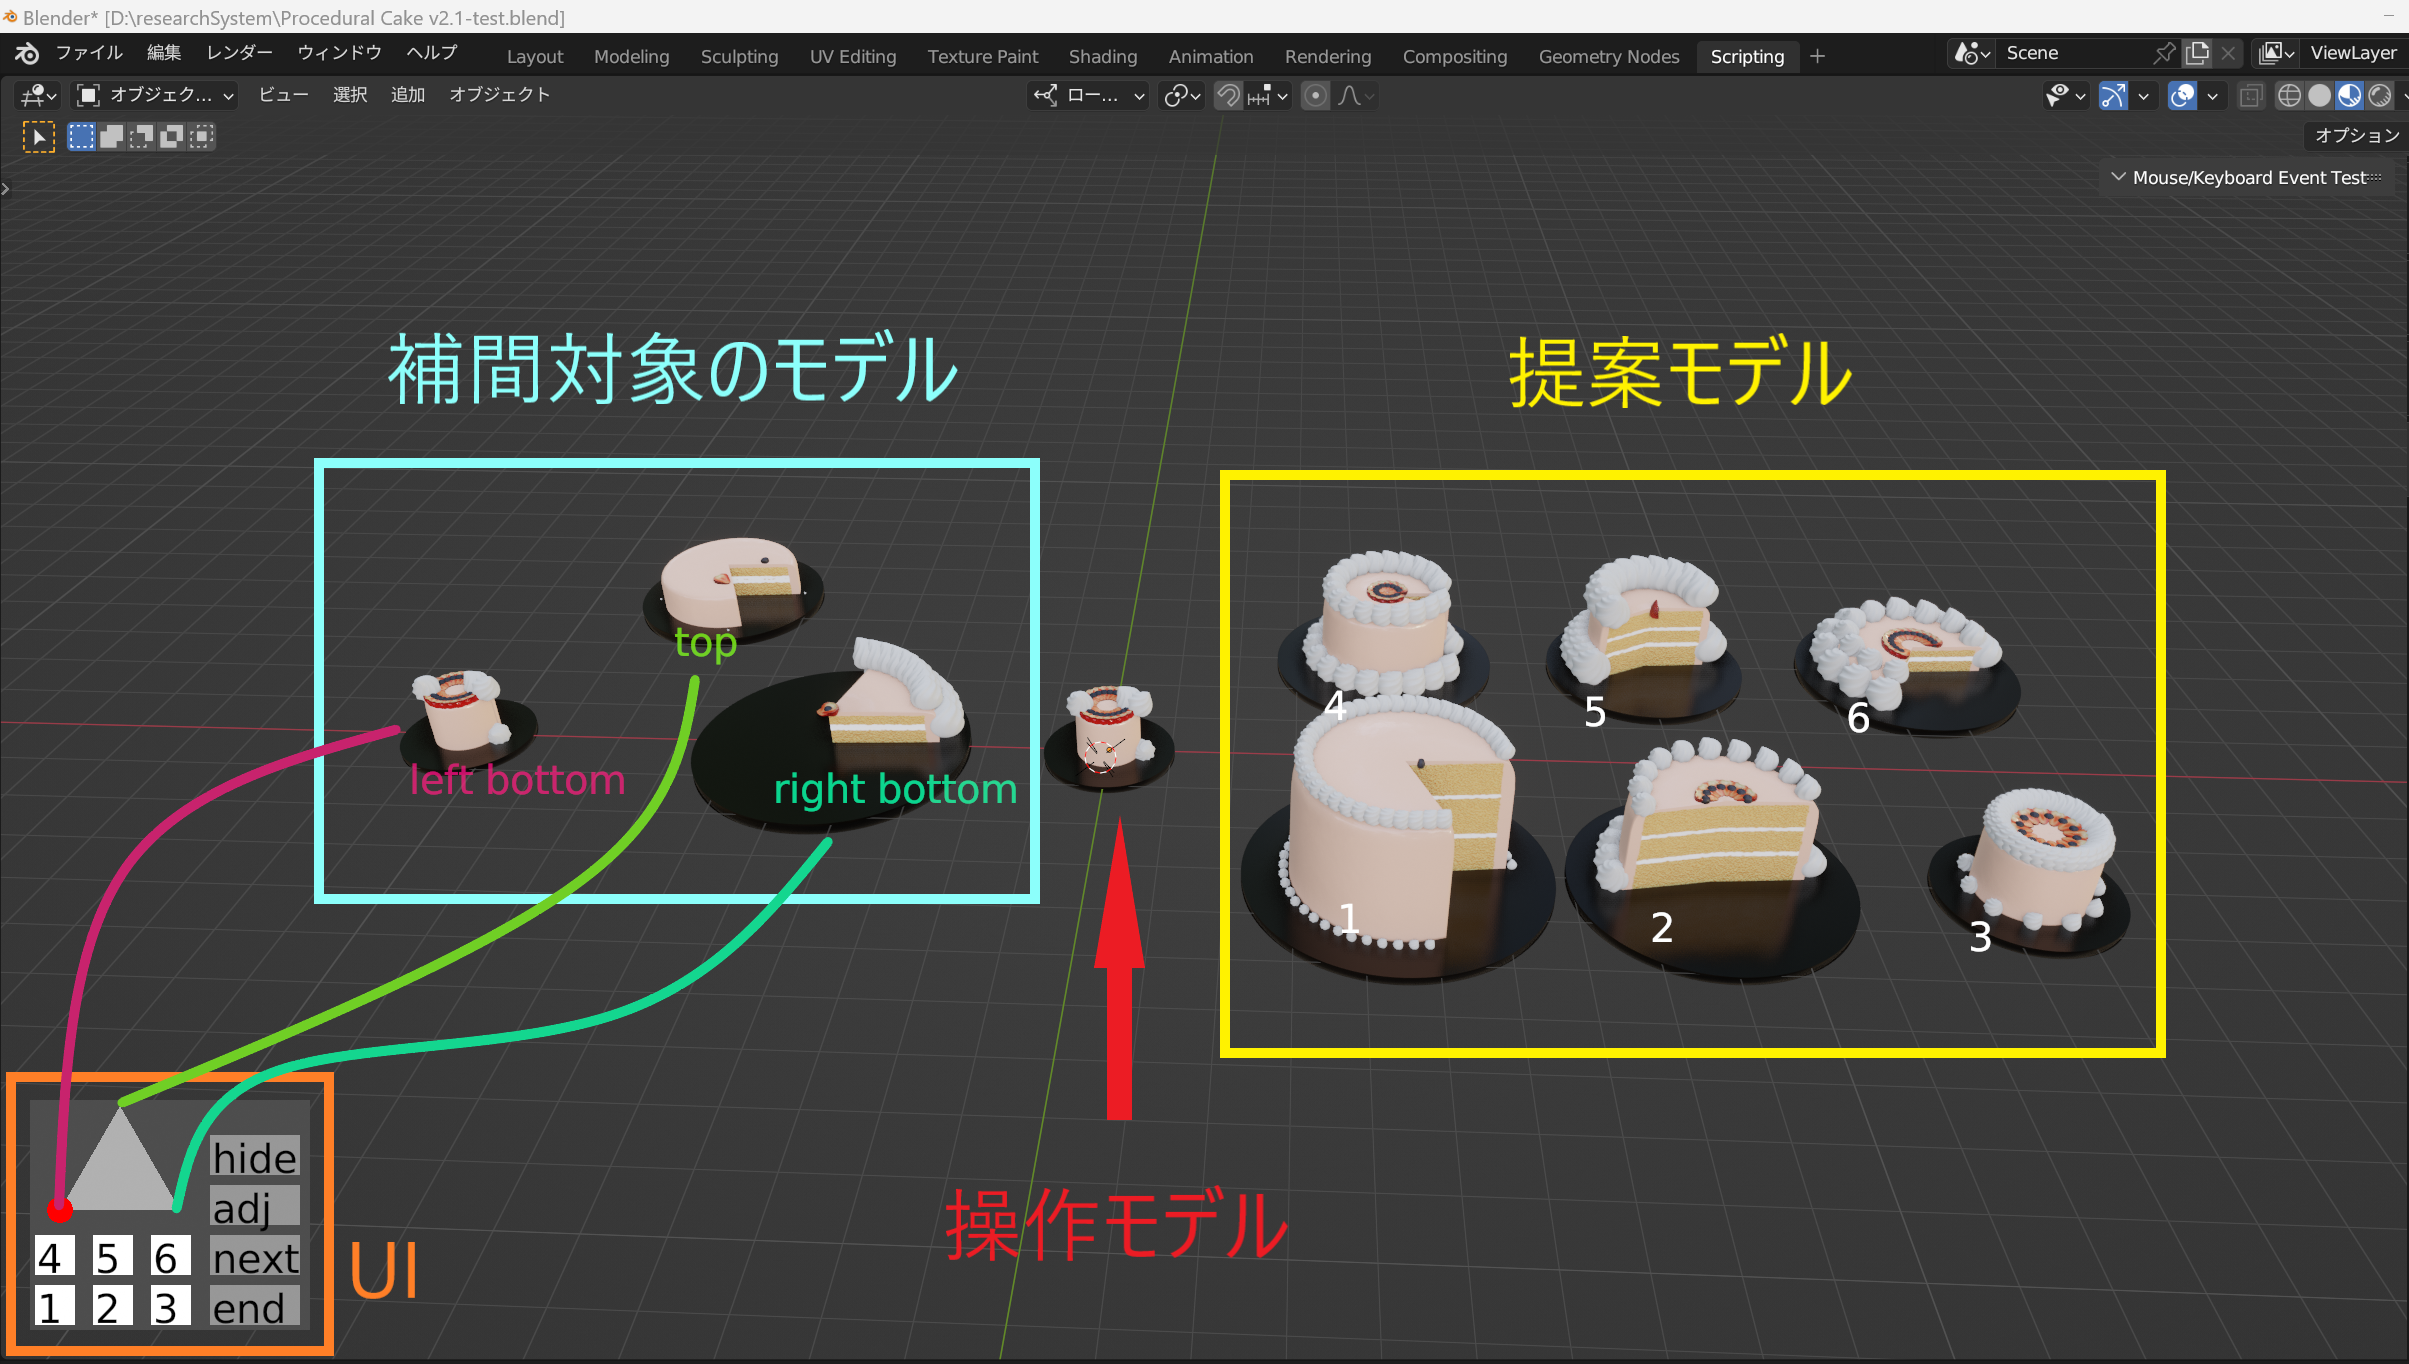
\includegraphics[width=0.8\hsize]{imgs/system_ano.png}
  \figcaption{\small 実装したシステム}
  \label{system}
\end{minipage}\\ \\
 %\vspace{7mm}

 
    \begin{minipage}[b]{0.35\hsize}
      \centering
      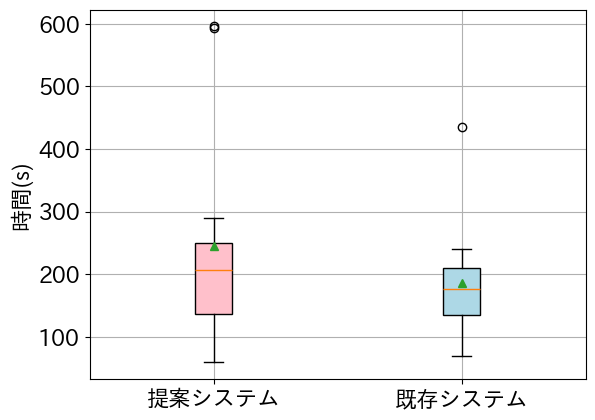
\includegraphics[width=0.8\hsize]{./imgs/sofaAllTime.png}
            \figcaption{全時間}\label{fig:exp2AllTime}
     \end{minipage}
     \begin{minipage}[b]{0.35\hsize}
      \centering
      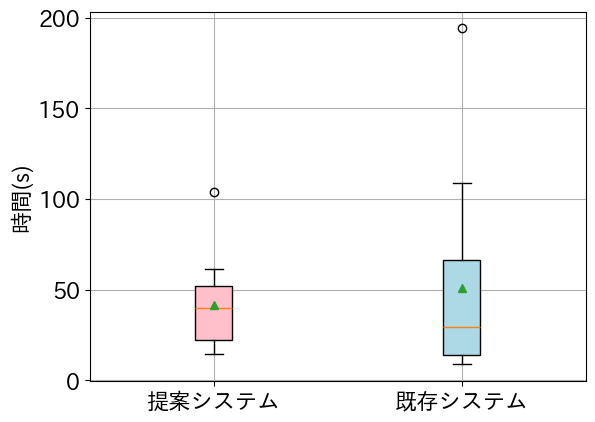
\includegraphics[width=0.8\hsize]{./imgs/sofaStepTime.png}
            \figcaption{1ステップ当たりの時間}\label{fig:exp2StepTime}
     \end{minipage}
     \begin{minipage}[b]{0.35\hsize}
      \centering
      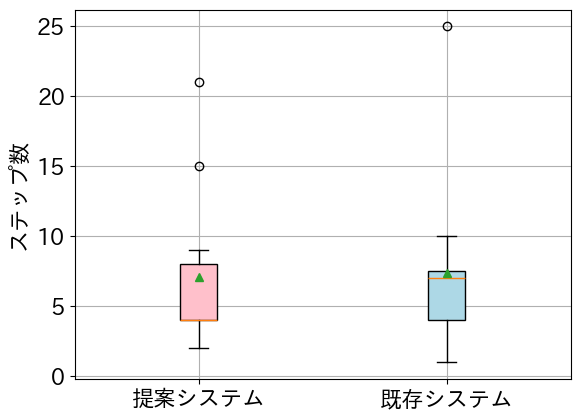
\includegraphics[width=0.8\hsize]{./imgs/sofaStepCnt.png}
            \figcaption{ステップ数}\label{fig:exp2StepNum}
     \end{minipage}
 \\
 
 \begin{minipage}{1\hsize}
\vspace{-1mm}
  \centering
  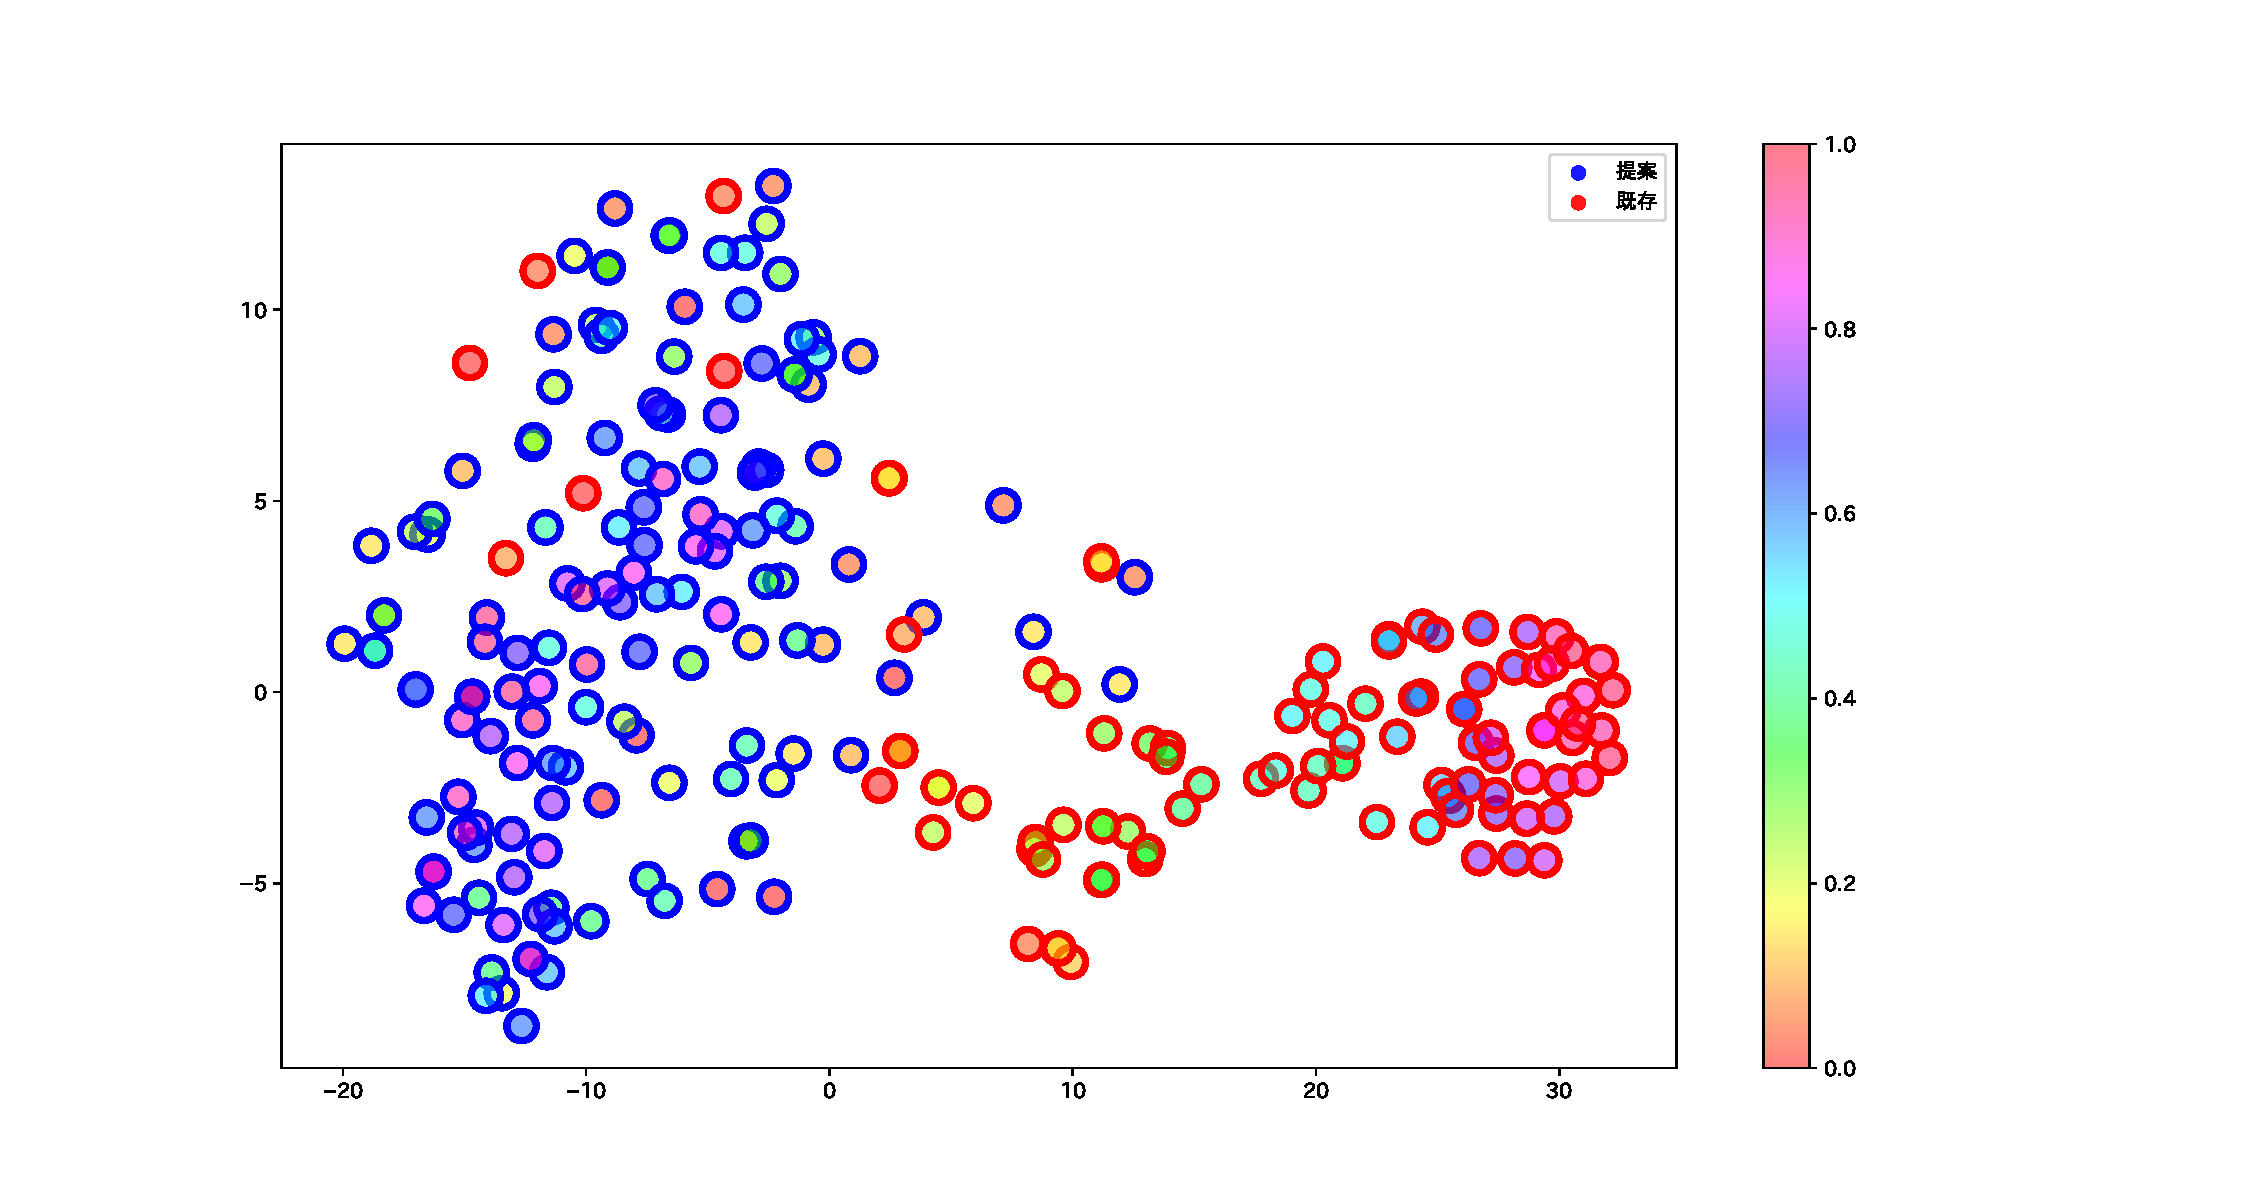
\includegraphics[angle=0, width=0.8\hsize]{imgs/sofa_5_tSNE.pdf}
  \figcaption{\small  パラメータの二次元可視化}
  \label{tSNE}
 \end{minipage}
\end{figure}


\noindent{\bf [Keywords]}
\indent
プロシージャルモデリング, インタラクティブ遺伝的アルゴリズム
\end{document}
